\documentclass{article}

% content/resources/templates/preamble.tex
\usepackage[margin=0.6in]{geometry}
\author{Milav Dabgar}
\usepackage{amsmath,amssymb,amsthm}
\usepackage{booktabs}
\usepackage{multirow}
\usepackage{xcolor}
\usepackage{tcolorbox}
\tcbuselibrary{breakable,skins}
\usepackage[colorlinks=true,linkcolor=blue]{hyperref}
\usepackage{titlesec}
\usepackage{enumitem}
\usepackage{tikz}
\usepackage{pgfplots}
\usepackage{circuitikz}
\usepackage[version=4]{mhchem}
\usepackage{longtable}
\usepackage{array}
\usepackage{float}
\usepackage{caption}
\usepackage{listings}

\lstset{
  basicstyle=\small\ttfamily,
  breaklines=true,
  breakatwhitespace=false,
  postbreak=\mbox{\textcolor{red}{$\hookrightarrow$}\space},
  float=false,
  numbers=left,
  numberstyle=\tiny\color{gray},
  numbersep=10pt,
  xleftmargin=2em,
  keywordstyle=\color{blue},
  commentstyle=\color{green!60!black},
  stringstyle=\color{purple},
  backgroundcolor=\color{gray!5},
  showstringspaces=false,
  tabsize=2,
  captionpos=b,
  keepspaces=true,
  columns=flexible
}

\pgfplotsset{compat=1.18}
\usetikzlibrary{shapes,arrows,positioning,calc,patterns,decorations.pathmorphing,decorations.markings,arrows.meta}

% Color scheme
\definecolor{headcolor}{RGB}{0,102,204}
\definecolor{keycolor}{RGB}{220,20,60}
\definecolor{solutioncolor}{RGB}{34,139,34}
\definecolor{mnemoniccolor}{RGB}{148,0,211}
\definecolor{codecolor}{RGB}{0,0,100}

% Spacing
\setlength{\parskip}{3pt}
\setlist[itemize]{nosep}
\setlist[enumerate]{nosep}

% Title formatting
\titleformat{\section}{\Large\bfseries\color{headcolor}}{\thesection}{1em}{}
\titleformat{\subsection}{\large\bfseries\color{headcolor}}{\thesubsection}{1em}{}

% Pandoc tightlist compatibility
\providecommand{\tightlist}{%
  \setlength{\itemsep}{0pt}\setlength{\parskip}{0pt}}

% Pandoc longtable compatibility
\newcounter{none}
\def\thenone{}


% content/resources/templates/english-boxes.tex

% Custom environments
\newtcolorbox{solutionbox}{
 breakable,
 enhanced,
 colback=solutioncolor!5!white,
 colframe=solutioncolor!75!black,
 fonttitle=\bfseries,
 title=Solution
}

\newtcolorbox{solutionboxnobreak}{
 colback=solutioncolor!5!white,
 colframe=solutioncolor!75!black,
 fonttitle=\bfseries,
 title=Solution
}

\newtcolorbox{keyformula}{
 breakable,
 enhanced,
 colback=keycolor!5!white,
 colframe=keycolor!75!black,
 fonttitle=\bfseries,
 title=Key Formula
}

\newtcolorbox{mnemonicboxenv}{
 breakable,
 enhanced,
 colback=mnemoniccolor!5!white,
 colframe=mnemoniccolor!75!black,
 fonttitle=\bfseries,
 title=Mnemonic
}

\newcommand{\mnemonicbox}[1]{%
  \begin{mnemonicboxenv}
    #1
  \end{mnemonicboxenv}
}


% Custom commands for GTU solutions
% This file defines semantic commands for consistent formatting

% Question command with automatic formatting
\newcommand{\question}[2]{%
  \section*{Question #1}%
  \textbf{#2}%
}

% OR question variant
\newcommand{\questionor}[2]{%
  \section*{Question #1 OR}%
  \textbf{#2}%
}

% Proper table environment with caption
\newenvironment{answertable}[1]{%
  \begin{table}[htbp]
  \centering
  \caption{#1}
}{%
  \end{table}
}

% Proper figure environment for diagrams
\newenvironment{answerdiagram}[1]{%
  \begin{figure}[htbp]
  \centering
  \caption{#1}
}{%
  \end{figure}
}

% Semantic markup for key terms
\newcommand{\keyword}[1]{\textbf{#1}}
\newcommand{\code}[1]{\texttt{#1}}
\newcommand{\classname}[1]{\texttt{#1}}
\newcommand{\methodname}[1]{\texttt{#1}}

% Proper quotation marks
\newcommand{\mnemonic}[1]{``#1''}


\title{Digital Electronics (4321102) - Summer 2023 Solution}
\date{August 07, 2023}

\begin{document}
\maketitle

\questionmarks{1(a)}{3}{Explain De-Morgan's theorem for Boolean algebra}


\begin{solutionbox}
De-Morgan's theorem consists of two laws that show the relationship between AND, OR, and NOT operations:

\textbf{Law 1}: The complement of a sum equals the product of complements
\[ \overline{A + B} = \overline{A} \cdot \overline{B} \]

\textbf{Law 2}: The complement of a product equals the sum of complements
\[ \overline{A \cdot B} = \overline{A} + \overline{B} \]

\captionof{table}{De-Morgan's Laws Verification}
\begin{center}
\begin{tabulary}{\linewidth}{|C|C|C|C|C|C|C|}
\hline
A & B & A+B & $\overline{A+B}$ & $\overline{A}$ & $\overline{B}$ & $\overline{A}\cdot\overline{B}$ \\
\hline
0 & 0 & 0 & 1 & 1 & 1 & 1 \\
\hline
0 & 1 & 1 & 0 & 1 & 0 & 0 \\
\hline
1 & 0 & 1 & 0 & 0 & 1 & 0 \\
\hline
1 & 1 & 1 & 0 & 0 & 0 & 0 \\
\hline
\end{tabulary}
\end{center}
\end{solutionbox}
\mnemonicbox{"NOT over OR becomes AND of NOTs, NOT over AND becomes OR of NOTs"}

\questionmarks{1(b)}{4}{Convert following decimal number into binary and octal number (i) 215 (ii) 59}


\begin{solutionbox}
\textbf{Binary Conversion:}

\textbf{For 215:}
\begin{itemize}
\item Divide by 2 repeatedly: $215/2 = 107$ remainder 1
\item $107/2 = 53$ remainder 1
\item $53/2 = 26$ remainder 1
\item $26/2 = 13$ remainder 0
\item $13/2 = 6$ remainder 1
\item $6/2 = 3$ remainder 0
\item $3/2 = 1$ remainder 1
\item $1/2 = 0$ remainder 1
\item Therefore, $(215)_{10} = (11010111)_2$
\end{itemize}

\textbf{For 59:}
\begin{itemize}
\item Divide by 2 repeatedly: $59/2 = 29$ remainder 1
\item $29/2 = 14$ remainder 1
\item $14/2 = 7$ remainder 0
\item $7/2 = 3$ remainder 1
\item $3/2 = 1$ remainder 1
\item $1/2 = 0$ remainder 1
\item Therefore, $(59)_{10} = (111011)_2$
\end{itemize}

\textbf{Octal Conversion:}

\textbf{For 215:}
\begin{itemize}
\item Divide by 8 repeatedly: $215/8 = 26$ remainder 7
\item $26/8 = 3$ remainder 2
\item $3/8 = 0$ remainder 3
\item Therefore, $(215)_{10} = (327)_8$
\end{itemize}

\textbf{For 59:}
\begin{itemize}
\item Divide by 8 repeatedly: $59/8 = 7$ remainder 3
\item $7/8 = 0$ remainder 7
\item Therefore, $(59)_{10} = (73)_8$
\end{itemize}

\captionof{table}{Number Conversion Summary}
\begin{center}
\begin{tabulary}{\linewidth}{|L|L|L|}
\hline
Decimal & Binary & Octal \\
\hline
215 & 11010111 & 327 \\
\hline
59 & 111011 & 73 \\
\hline
\end{tabulary}
\end{center}
\end{solutionbox}
\mnemonicbox{"Divide by base, read remainders bottom-up"}

\questionmarks{1(c)(I)}{2}{Write the base of decimal, binary, octal and hexadecimal number system}


\begin{solutionbox}
\captionof{table}{Number System Bases}
\begin{center}
\begin{tabulary}{\linewidth}{|L|L|}
\hline
Number System & Base \\
\hline
Decimal & 10 \\
\hline
Binary & 2 \\
\hline
Octal & 8 \\
\hline
Hexadecimal & 16 \\
\hline
\end{tabulary}
\end{center}
\end{solutionbox}
\mnemonicbox{"D-B-O-H: 10-2-8-16"}

\questionmarks{1(c)(II)}{2}{$(147)_{10} = (\_\_\_\_\_\_\_\_\_\_\_\_)_2 = (\_\_\_\_\_\_\_\_\_\_\_\_\_\_)_{16}$}


\begin{solutionbox}
\textbf{Decimal to Binary conversion:}
\begin{itemize}
\item $147/2 = 73$ remainder 1
\item $73/2 = 36$ remainder 1
\item $36/2 = 18$ remainder 0
\item $18/2 = 9$ remainder 0
\item $9/2 = 4$ remainder 1
\item $4/2 = 2$ remainder 0
\item $2/2 = 1$ remainder 0
\item $1/2 = 0$ remainder 1
\item Therefore, $(147)_{10} = (10010011)_2$
\end{itemize}

\textbf{Decimal to Hexadecimal conversion:}
\begin{itemize}
\item Group binary digits in sets of 4: 1001 0011
\item Convert each group to hex: $1001 = 9$, $0011 = 3$
\item Therefore, $(147)_{10} = (93)_{16}$
\end{itemize}

\captionof{table}{Conversion Result}
\begin{center}
\begin{tabulary}{\linewidth}{|L|L|L|}
\hline
Decimal & Binary & Hexadecimal \\
\hline
147 & 10010011 & 93 \\
\hline
\end{tabulary}
\end{center}
\end{solutionbox}
\mnemonicbox{"Group by 4 from right for hex"}

\questionmarks{1(c)(III)}{3}{Convert following binary code into grey code (i) 1011 (ii) 1110}


\begin{solutionbox}
\textbf{Binary to Gray code conversion procedure:}
\begin{enumerate}
\item The MSB (leftmost bit) of the Gray code is the same as the MSB of the binary code
\item Other bits of the Gray code are obtained by XORing adjacent bits of the binary code
\end{enumerate}

\textbf{For 1011:}
\begin{itemize}
\item MSB of Gray = MSB of Binary = 1
\item Second bit = $1 \oplus 0 = 1$
\item Third bit = $0 \oplus 1 = 1$
\item Fourth bit = $1 \oplus 1 = 0$
\item Therefore, $(1011)_2 = (1110)_{gray}$
\end{itemize}

\textbf{For 1110:}
\begin{itemize}
\item MSB of Gray = MSB of Binary = 1
\item Second bit = $1 \oplus 1 = 0$
\item Third bit = $1 \oplus 1 = 0$
\item Fourth bit = $1 \oplus 0 = 1$
\item Therefore, $(1110)_2 = (1001)_{gray}$
\end{itemize}

\captionof{table}{Binary to Gray Code Conversion}
\begin{center}
\begin{tabulary}{\linewidth}{|L|L|L|}
\hline
Binary & Step-by-step & Gray Code \\
\hline
1011 & 1, $1\oplus0=1$, $0\oplus1=1$, $1\oplus1=0$ & 1110 \\
\hline
1110 & 1, $1\oplus1=0$, $1\oplus1=0$, $1\oplus0=1$ & 1001 \\
\hline
\end{tabulary}
\end{center}
\end{solutionbox}
\mnemonicbox{"Keep first, XOR the rest"}

\questionmarks{1(c) [OR] (I)}{2}{Write the full form of BCD and ASCII}


\begin{solutionbox}
\captionof{table}{Full Forms of BCD and ASCII}
\begin{center}
\begin{tabulary}{\linewidth}{|L|L|}
\hline
Abbreviation & Full Form \\
\hline
BCD & Binary Coded Decimal \\
\hline
ASCII & American Standard Code for Information Interchange \\
\hline
\end{tabulary}
\end{center}
\end{solutionbox}
\mnemonicbox{"Binary Codes Decimal values, American Standards Code Information"}

\questionmarks{1(c) [OR] (II)}{2}{Write 1's and 2's complement of following binary numbers: (i) 1010 (ii) 1011}


\begin{solutionbox}
\textbf{1's Complement:} Invert all bits (change 0 to 1 and 1 to 0) \\
\textbf{2's Complement:} Take 1's complement and add 1

\textbf{For 1010:}
\begin{itemize}
\item 1's complement: 0101
\item 2's complement: $0101 + 1 = 0110$
\end{itemize}

\textbf{For 1011:}
\begin{itemize}
\item 1's complement: 0100
\item 2's complement: $0100 + 1 = 0101$
\end{itemize}

\captionof{table}{Complement Results}
\begin{center}
\begin{tabulary}{\linewidth}{|L|L|L|}
\hline
Binary & 1's Complement & 2's Complement \\
\hline
1010 & 0101 & 0110 \\
\hline
1011 & 0100 & 0101 \\
\hline
\end{tabulary}
\end{center}
\end{solutionbox}
\mnemonicbox{"Flip all bits for 1's, Add one more for 2's"}

\questionmarks{1(c) [OR] (III)}{3}{Perform subtraction using 2's complement method (i) $(110110)_2 - (101010)_2$}


\begin{solutionbox}
To subtract using 2's complement method:
\begin{enumerate}
\item Find 2's complement of subtrahend
\item Add it to the minuend
\item Discard any carry beyond the bit width
\end{enumerate}

\textbf{Subtraction: $(110110)_2 - (101010)_2$}

\textbf{Step 1:} Find 2's complement of 101010
\begin{itemize}
\item 1's complement of 101010 = 010101
\item 2's complement = $010101 + 1 = 010110$
\end{itemize}

\textbf{Step 2:} Add $110110 + 010110$

\begin{verbatim}
  1 1 1 1 1
  1 1 0 1 1 0
+ 0 1 0 1 1 0
--------------
  0 0 1 1 0 0
\end{verbatim}

\textbf{Step 3:} Result is $001100 = (12)_{10}$

\captionof{table}{Subtraction Process}
\begin{center}
\begin{tabulary}{\linewidth}{|C|L|L|}
\hline
Step & Operation & Result \\
\hline
1 & 2's complement of 101010 & 010110 \\
\hline
2 & Add $110110 + 010110$ & 001100 \\
\hline
3 & Final result (decimal) & 12 \\
\hline
\end{tabulary}
\end{center}
\end{solutionbox}
\mnemonicbox{"Complement the subtracted, add them up, carry goes away"}

\questionmarks{2(a)}{3}{Draw logic circuit of AND, OR and NOT gate using NAND gate only}


\begin{solutionbox}
\textbf{AND gate using NAND gates:}
\begin{itemize}
\item AND gate = NAND gate followed by NOT gate (NAND gate)
\end{itemize}

\textbf{OR gate using NAND gates:}
\begin{itemize}
\item OR gate = Apply NOT (NAND gate) to both inputs, then NAND those results
\end{itemize}

\textbf{NOT gate using NAND gate:}
\begin{itemize}
\item NOT gate = NAND gate with both inputs tied together
\end{itemize}

\begin{figure}[H]
\centering
\begin{circuitikz}[scale=0.8, transform shape]
% NOT Gate
\draw (0,4) node[nand port] (nand1) {};
\draw (nand1.in 1) -- ++(-0.5,0) node[left] {A};
\draw (nand1.in 2) -- ++(-0.5,0); 
\draw (nand1.out) -- ++(0.5,0) node[right] {NOT A};
\draw (nand1.in 1) -- (nand1.in 2); % Tie inputs

% AND Gate
\draw (5,4) node[nand port] (nand2) {};
\draw (7,4) node[nand port] (nand3) {};
\draw (nand2.in 1) -- ++(-0.5,0) node[left] {B};
\draw (nand2.in 2) -- ++(-0.5,0) node[left] {C};
\draw (nand2.out) -- (nand3.in 1);
\draw (nand2.out) -- (nand3.in 2); % Tie inputs of second NAND
\draw (nand3.out) -- ++(0.5,0) node[right] {B AND C};

% OR Gate
\draw (0,0) node[nand port] (nand4) {};
\draw (0,-2) node[nand port] (nand5) {};
\draw (3,-1) node[nand port] (nand6) {};
\draw (nand4.in 1) -- (nand4.in 2) -- ++(-0.5,0) node[left] {D};
\draw (nand5.in 1) -- (nand5.in 2) -- ++(-0.5,0) node[left] {E};
\draw (nand4.out) -- (nand6.in 1);
\draw (nand5.out) -- (nand6.in 2);
\draw (nand6.out) -- ++(0.5,0) node[right] {D OR E};

\node at (0,2.5) {\textbf{NOT Gate}};
\node at (6,2.5) {\textbf{AND Gate}};
\node at (1.5,-3) {\textbf{OR Gate}};
\end{circuitikz}
\caption{Universal Gates implementation}
\end{figure}
\end{solutionbox}
\mnemonicbox{"NAND alone for NOT, NAND twice for AND, NAND each then NAND again for OR"}

\questionmarks{2(b)}{4}{Draw/Write logic symbol, truth table and equation of following logic gates (i) XOR gate (ii) OR gate}


\begin{solutionbox}
\textbf{XOR Gate:}

\textbf{Logic Symbol:}
\begin{center}
\begin{circuitikz}
\draw (0,0) node[xor port] (xor) {};
\draw (xor.in 1) -- ++(-0.5,0) node[left] {A};
\draw (xor.in 2) -- ++(-0.5,0) node[left] {B};
\draw (xor.out) -- ++(0.5,0) node[right] {Y};
\end{circuitikz}
\end{center}

\textbf{Truth Table:}
\begin{center}
\begin{tabulary}{\linewidth}{|C|C|C|}
\hline
A & B & Y (A$\oplus$B) \\
\hline
0 & 0 & 0 \\
\hline
0 & 1 & 1 \\
\hline
1 & 0 & 1 \\
\hline
1 & 1 & 0 \\
\hline
\end{tabulary}
\end{center}

\textbf{Boolean Equation:} $Y = A \oplus B = A'B + AB'$

\textbf{OR Gate:}

\textbf{Logic Symbol:}
\begin{center}
\begin{circuitikz}
\draw (0,0) node[or port] (or) {};
\draw (or.in 1) -- ++(-0.5,0) node[left] {A};
\draw (or.in 2) -- ++(-0.5,0) node[left] {B};
\draw (or.out) -- ++(0.5,0) node[right] {Y};
\end{circuitikz}
\end{center}

\textbf{Truth Table:}
\begin{center}
\begin{tabulary}{\linewidth}{|C|C|C|}
\hline
A & B & Y (A+B) \\
\hline
0 & 0 & 0 \\
\hline
0 & 1 & 1 \\
\hline
1 & 0 & 1 \\
\hline
1 & 1 & 1 \\
\hline
\end{tabulary}
\end{center}

\textbf{Boolean Equation:} $Y = A+B$
\end{solutionbox}
\mnemonicbox{"XOR: Exclusive OR - one or the other but not both; OR: one or the other or both"}

\questionmarks{2(c)(I)}{3}{Simplify the Boolean expression using algebraic method $Y = A + B[AC + (B + \overline{C})D]$}


\begin{solutionbox}
\textbf{Step-by-step simplification:}

\begin{align*}
Y &= A + B[AC + (B + \overline{C})D] \\
Y &= A + B[AC + BD + \overline{C}D] \\
Y &= A + BAC + BBD + B\overline{C}D \\
Y &= A + ABC + BD + B\overline{C}D & (\text{Since } BB = B) \\
Y &= A + AC + BD + B\overline{C}D & (\text{Absorption: } A + AB = A) \\
Y &= A + BD + B\overline{C}D & (\text{Absorption: } A + AC = A) \\
Y &= A + BD(1 + \overline{C}) \\
Y &= A + BD & (\text{Since } 1 + X = 1)
\end{align*}

\textbf{Final expression:} $Y = A + BD$

\captionof{table}{Simplification Steps}
\begin{center}
\begin{tabulary}{\linewidth}{|C|L|L|}
\hline
Step & Expression & Law Applied \\
\hline
1 & $A + B[AC + (B + \overline{C})D]$ & Initial \\
\hline
2 & $A + B[AC + BD + \overline{C}D]$ & Distributive \\
\hline
3 & $A + BAC + BBD + B\overline{C}D$ & Distributive \\
\hline
4 & $A + ABC + BD + B\overline{C}D$ & Idempotent ($BB = B$) \\
\hline
5 & $A + AC + BD + B\overline{C}D$ & Absorption \\
\hline
6 & $A + BD + B\overline{C}D$ & Absorption ($A+AC=A$) \\
\hline
7 & $A + BD(1 + \overline{C})$ & Factoring \\
\hline
8 & $A + BD$ & Identity law \\
\hline
\end{tabulary}
\end{center}
\end{solutionbox}
\mnemonicbox{"Always look for idempotence, absorption, and complement patterns"}

\questionmarks{2(c)(II)}{4}{Simplify the Boolean expression using Karnaugh Map F(A,B,C) = $\Sigma m(0, 2, 3, 4, 5, 6)$}


\begin{solutionbox}
\textbf{K-map for $F(A,B,C) = \Sigma m(0, 2, 3, 4, 5, 6)$:}

\begin{center}
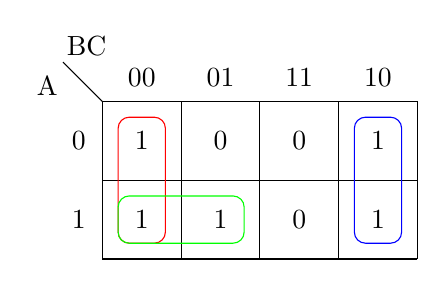
\begin{tikzpicture}
\draw (0,0) grid (4,2);
\draw (0,2) -- (-0.5,2.5);
\node at (-0.7,2.2) {A};
\node at (-0.2,2.7) {BC};
\node at (0.5,2.3) {00};
\node at (1.5,2.3) {01};
\node at (2.5,2.3) {11};
\node at (3.5,2.3) {10};
\node at (-0.3,1.5) {0};
\node at (-0.3,0.5) {1};

% Cell values
\node at (0.5,1.5) {1}; % 0
\node at (1.5,1.5) {0}; % 1
\node at (2.5,1.5) {0}; % 3
\node at (3.5,1.5) {1}; % 2
\node at (0.5,0.5) {1}; % 4
\node at (1.5,0.5) {1}; % 5
\node at (2.5,0.5) {0}; % 7
\node at (3.5,0.5) {1}; % 6

% Groupings
\draw[red, rounded corners] (0.2,1.8) rectangle (0.8,0.2); % 0,4
\draw[blue, rounded corners] (3.2,1.8) rectangle (3.8,0.2); % 2,6
\draw[green, rounded corners] (0.2,0.2) rectangle (1.8,0.8); % 4,5
\end{tikzpicture}
\end{center}

\textbf{Group the 1s:}
\begin{itemize}
\item Group 1: m(0,4) - corresponds to $B'C'$
\item Group 2: m(2,6) - corresponds to $BC'$
\item Group 3: m(4,5) - corresponds to $AB'$
\end{itemize}

\textbf{Simplified expression:} $F(A,B,C) = B'C' + BC' + AB'$

\textbf{Result:}
$F = C'(B'+B) + AB' = C' + AB'$
\end{solutionbox}
\mnemonicbox{"Group adjacent 1s in powers of 2"}

\questionmarks{2 [OR] (a)}{3}{Draw logic circuit of AND, OR and NOT gate using NOR gate only}


\begin{solutionbox}
\textbf{NOT gate using NOR gate:}
\begin{itemize}
\item NOT gate = NOR gate with both inputs tied together
\end{itemize}

\textbf{AND gate using NOR gates:}
\begin{itemize}
\item AND gate = Apply NOT (NOR gate) to both inputs, then NOR those results again
\end{itemize}

\textbf{OR gate using NOR gates:}
\begin{itemize}
\item OR gate = NOR gate followed by NOT gate (NOR gate)
\end{itemize}

\begin{figure}[H]
\centering
\begin{circuitikz}[scale=0.8, transform shape]
% NOT Gate
\draw (0,4) node[nor port] (nor1) {};
\draw (nor1.in 1) -- ++(-0.5,0) node[left] {A};
\draw (nor1.in 2) -- ++(-0.5,0);
\draw (nor1.in 1) -- (nor1.in 2);
\draw (nor1.out) -- ++(0.5,0) node[right] {NOT A};

% AND Gate
\draw (0,0) node[nor port] (nor2) {};
\draw (0,-2) node[nor port] (nor3) {};
\draw (3,-1) node[nor port] (nor4) {};
\draw (nor2.in 1) -- (nor2.in 2) -- ++(-0.5,0) node[left] {B};
\draw (nor3.in 1) -- (nor3.in 2) -- ++(-0.5,0) node[left] {C};
\draw (nor2.out) -- (nor4.in 1);
\draw (nor3.out) -- (nor4.in 2);
\draw (nor4.out) -- ++(0.5,0) node[right] {B AND C};

% OR Gate
\draw (5,4) node[nor port] (nor5) {};
\draw (7,4) node[nor port] (nor6) {};
\draw (nor5.in 1) -- ++(-0.5,0) node[left] {D};
\draw (nor5.in 2) -- ++(-0.5,0) node[left] {E};
\draw (nor5.out) -- (nor6.in 1);
\draw (nor5.out) -- (nor6.in 2);
\draw (nor6.out) -- ++(0.5,0) node[right] {D OR E};

\node at (0,2.5) {\textbf{NOT Gate}};
\node at (1.5,-3) {\textbf{AND Gate}};
\node at (6,2.5) {\textbf{OR Gate}};
\end{circuitikz}
\caption{Universal Gates implementation (NOR)}
\end{figure}
\end{solutionbox}
\mnemonicbox{"NOR alone for NOT, NOT each then NOR for AND, Double NOR for OR"}

\questionmarks{2 [OR] (b)}{4}{Draw/Write logic symbol, truth table and equation of following logic gates (i) NOR gate (ii) AND gate}


\begin{solutionbox}
\textbf{NOR Gate:}

\textbf{Logic Symbol:}
\begin{center}
\begin{circuitikz}
\draw (0,0) node[nor port] (nor) {};
\draw (nor.in 1) -- ++(-0.5,0) node[left] {A};
\draw (nor.in 2) -- ++(-0.5,0) node[left] {B};
\draw (nor.out) -- ++(0.5,0) node[right] {Y};
\end{circuitikz}
\end{center}

\textbf{Truth Table:}
\begin{center}
\begin{tabulary}{\linewidth}{|C|C|C|}
\hline
A & B & Y (A+B)' \\
\hline
0 & 0 & 1 \\
\hline
0 & 1 & 0 \\
\hline
1 & 0 & 0 \\
\hline
1 & 1 & 0 \\
\hline
\end{tabulary}
\end{center}

\textbf{Boolean Equation:} $Y = (A+B)' = A'B'$

\textbf{AND Gate:}

\textbf{Logic Symbol:}
\begin{center}
\begin{circuitikz}
\draw (0,0) node[and port] (and) {};
\draw (and.in 1) -- ++(-0.5,0) node[left] {A};
\draw (and.in 2) -- ++(-0.5,0) node[left] {B};
\draw (and.out) -- ++(0.5,0) node[right] {Y};
\end{circuitikz}
\end{center}

\textbf{Truth Table:}
\begin{center}
\begin{tabulary}{\linewidth}{|C|C|C|}
\hline
A & B & Y (A$\cdot$B) \\
\hline
0 & 0 & 0 \\
\hline
0 & 1 & 0 \\
\hline
1 & 0 & 0 \\
\hline
1 & 1 & 1 \\
\hline
\end{tabulary}
\end{center}

\textbf{Boolean Equation:} $Y = A \cdot B$
\end{solutionbox}
\mnemonicbox{"NOR: NOT OR - neither one nor the other; AND: both must be 1"}

\questionmarks{2 [OR] (c)}{7}{Write the Boolean expression of Q for above logic circuit. Simplify the Boolean expression of Q and draw the logic circuit of simplified circuit using AND-OR-Invert method}


\begin{solutionbox}
\textbf{Step 1:} Write Boolean expression from the circuit:
$Q = (A + B) \cdot (B + C \cdot ((B + C)'))$ \\
$Q = (A + B) \cdot (B + C \cdot (B' \cdot C'))$ \\
$Q = (A + B) \cdot (B + C \cdot B' \cdot C')$

\textbf{Step 2:} Simplify the expression:
\begin{itemize}
\item Note that $C \cdot C' = 0$
\item Therefore, $C \cdot B' \cdot C' = 0$
\item So $Q = (A + B) \cdot (B + 0) = (A + B) \cdot B = A \cdot B + B \cdot B = A \cdot B + B = B + A \cdot B = B(1 + A) = B$
\end{itemize}

\textbf{Step 3:} Final simplified expression: $Q = B$

\textbf{Step 4:} AND-OR-Invert implementation of $Q = B$:
\begin{itemize}
\item This is simply a wire from input B to output Q
\end{itemize}

\begin{center}
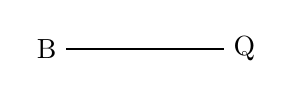
\begin{tikzpicture}
\draw (0,0) node[left] {B} -- (2,0) node[right] {Q};
\end{tikzpicture}
\end{center}

\captionof{table}{Simplification Steps}
\begin{center}
\begin{tabulary}{\linewidth}{|C|L|L|}
\hline
Step & Expression & Simplification \\
\hline
1 & $(A + B) \cdot (B + C \cdot ((B + C)'))$ & Original expression \\
\hline
2 & $(A + B) \cdot (B + C \cdot B' \cdot C')$ & Applying De Morgan's \\
\hline
3 & $(A + B) \cdot (B + 0)$ & $C \cdot C' = 0$ \\
\hline
4 & $(A + B) \cdot B$ & Simplifying \\
\hline
5 & $A \cdot B + B \cdot B$ & Distributive property \\
\hline
6 & $A \cdot B + B$ & Idempotent property ($B \cdot B=B$) \\
\hline
7 & $B(1 + A)$ & Factoring \\
\hline
8 & $B$ & $1 + A = 1$ \\
\hline
\end{tabulary}
\end{center}
\end{solutionbox}
\mnemonicbox{"When complementary variables multiply, they zero out"}

\questionmarks{3(a)}{3}{Define combinational circuit. Give two examples of combinational circuits}


\begin{solutionbox}
\textbf{Combinational circuit:} A digital circuit whose output depends only on the current input values and not on previous inputs or states. In combinational circuits, there is no memory or feedback.

\textbf{Key characteristics:}
\begin{itemize}
\item Output depends only on current inputs
\item No memory elements
\item No feedback paths
\end{itemize}

\textbf{Examples of combinational circuits:}
\begin{enumerate}
\item Multiplexers (MUX)
\item Decoders
\item Adders/Subtractors
\item Encoders
\item Comparators
\end{enumerate}

\captionof{table}{Combinational vs Sequential Circuits}
\begin{center}
\begin{tabulary}{\linewidth}{|L|L|L|}
\hline
Characteristic & Combinational Circuit & Sequential Circuit \\
\hline
Memory & No & Yes \\
\hline
Feedback & No & Usually \\
\hline
Output depends on & Current inputs only & Current and previous inputs \\
\hline
Examples & Multiplexers, Adders & Flip-flops, Counters \\
\hline
\end{tabulary}
\end{center}
\end{solutionbox}
\mnemonicbox{"Combinational circuits: Current In, Current Out - no memory about"}

\questionmarks{3(b)}{4}{Explain half adder using logic circuit and truth table}


\begin{solutionbox}
\textbf{Half Adder:} A combinational circuit that adds two binary digits and produces sum and carry outputs.

\textbf{Logic Circuit:}
\begin{center}
\begin{circuitikz}
\draw (0,2) node[xor port] (xor) {};
\draw (0,0) node[and port] (and) {};
\draw (xor.in 1) -- ++(-1,0) node[left] (A) {A};
\draw (xor.in 2) -- ++(-1,0) node[left] (B) {B};
\draw (A) |- (and.in 1);
\draw (B) |- (and.in 2);
\draw (xor.out) -- ++(1,0) node[right] {Sum};
\draw (and.out) -- ++(1,0) node[right] {Carry};
\end{circuitikz}
\end{center}

\textbf{Truth Table:}
\begin{center}
\begin{tabulary}{\linewidth}{|C|C|C|C|}
\hline
A & B & Sum & Carry \\
\hline
0 & 0 & 0 & 0 \\
\hline
0 & 1 & 1 & 0 \\
\hline
1 & 0 & 1 & 0 \\
\hline
1 & 1 & 0 & 1 \\
\hline
\end{tabulary}
\end{center}

\textbf{Boolean Equations:}
\begin{itemize}
\item Sum = $A \oplus B = A'B + AB'$
\item Carry = $A \cdot B$
\end{itemize}

\textbf{Limitations:}
\begin{itemize}
\item Cannot add three binary digits
\item Cannot accommodate carry input from previous stage
\end{itemize}
\end{solutionbox}
\mnemonicbox{"XOR for Sum, AND for Carry"}

\questionmarks{3(c)(I)}{3}{Explain multiplexer in brief}


\begin{solutionbox}
\textbf{Multiplexer (MUX):} A combinational circuit that selects one of several input signals and forwards it to a single output line based on select lines.

\textbf{Key features:}
\begin{itemize}
\item Acts as a digital switch
\item Has $2^n$ data inputs, $n$ select lines, and 1 output
\item Select lines determine which input is connected to output
\end{itemize}

\textbf{Common multiplexers:}
\begin{itemize}
\item 2:1 MUX (1 select line)
\item 4:1 MUX (2 select lines)
\item 8:1 MUX (3 select lines)
\end{itemize}

\textbf{Basic structure:}
\begin{center}
\begin{tikzpicture}[node distance=1.5cm]
\node [gtu input] (i0) {I0};
\node [gtu input, below of=i0] (i1) {I1};
\node [below of=i1] (dots) {...};
\node [gtu input, below of=dots] (in) {$I_{2^n-1}$};

\node [trapezium, draw, shape border rotate=270, minimum height=3cm, minimum width=2cm, right of=dots, xshift=2cm] (mux) {MUX};

\draw [gtu arrow] (i0) -- (mux.north west);
\draw [gtu arrow] (i1) -- (mux.west |- i1);
\draw [gtu arrow] (in) -- (mux.south west);

\node [gtu input, below of=mux, yshift=-1cm] (sel) {Select Lines};
\draw [gtu arrow] (sel) -- (mux.south);

\node [gtu output, right of=mux, xshift=2cm] (out) {Output Y};
\draw [gtu arrow] (mux.east) -- (out);

\end{tikzpicture}
\end{center}

\textbf{Applications:}
\begin{itemize}
\item Data routing
\item Data selection
\item Parallel to serial conversion
\item Implementation of Boolean functions
\end{itemize}
\end{solutionbox}
\mnemonicbox{"Many In, Selection picks, One Out"}

\questionmarks{3(c)(II)}{4}{Design 8:1 multiplexer. Write its truth table and draw its logic circuit}


\begin{solutionbox}
\textbf{8:1 Multiplexer Design:}
\begin{itemize}
\item 8 data inputs ($I_0$ to $I_7$)
\item 3 select lines ($S_2, S_1, S_0$)
\item 1 output (Y)
\end{itemize}

\textbf{Truth Table:}
\begin{center}
\begin{tabulary}{\linewidth}{|C|C|C|C|}
\hline
$S_2$ & $S_1$ & $S_0$ & Output Y \\
\hline
0 & 0 & 0 & $I_0$ \\
\hline
0 & 0 & 1 & $I_1$ \\
\hline
0 & 1 & 0 & $I_2$ \\
\hline
0 & 1 & 1 & $I_3$ \\
\hline
1 & 0 & 0 & $I_4$ \\
\hline
1 & 0 & 1 & $I_5$ \\
\hline
1 & 1 & 0 & $I_6$ \\
\hline
1 & 1 & 1 & $I_7$ \\
\hline
\end{tabulary}
\end{center}

\textbf{Boolean Equation:}
$Y = S_2'S_1'S_0'I_0 + S_2'S_1'S_0I_1 + S_2'S_1S_0'I_2 + S_2'S_1S_0I_3 + S_2S_1'S_0'I_4 + S_2S_1'S_0I_5 + S_2S_1S_0'I_6 + S_2S_1S_0I_7$

\textbf{Logic Circuit:}
\begin{center}
\begin{circuitikz}[scale=0.7, transform shape]
% AND Gates
\foreach \i in {0,...,7} {
    \draw (0, \i*1.5) node[and port, number inputs=4] (and\i) {};
    \draw (and\i.in 4) -- ++(-0.5,0) node[left] {$I_{\i}$};
}
% OR Gate
\draw (4, 5.25) node[or port, number inputs=8] (or) {};

% Connections to OR
\foreach \i [evaluate=\i as \j using int(\i+1)] in {0,...,7} {
    \draw (and\i.out) -- (or.in \j);
}
\node at (6, 5.25) {Y};
\draw (or.out) -- (6,5.25);
\end{circuitikz}
\end{center}
\end{solutionbox}
\mnemonicbox{"Eight inputs, three selects, decode and OR to output"}

\questionmarks{3 [OR] (a)}{3}{Draw the block diagram of 4-bit binary parallel adder}


\begin{solutionbox}
\textbf{4-bit Binary Parallel Adder:}
A circuit that adds two 4-bit binary numbers and produces a 4-bit sum and a carry output.

\begin{center}
\begin{tikzpicture}[node distance=2.5cm, auto]
 \node [gtu block] (fa0) {FA0};
 \node [gtu block, left of=fa0] (fa1) {FA1};
 \node [gtu block, left of=fa1] (fa2) {FA2};
 \node [gtu block, left of=fa2] (fa3) {FA3};

 % Inputs A and B
 \foreach \i in {0,1,2,3} {
  \draw [gtu arrow] ([yshift=0.5cm]fa\i.north) -- (fa\i.north) node[midway, right] {$A_\i, B_\i$};
  \draw [gtu arrow] (fa\i.south) -- ([yshift=-0.5cm]fa\i.south) node[midway, right] {$S_\i$};
 }

 % Carries
 \draw [gtu arrow] (fa0.west) -- (fa1.east) node[midway, above] {$C_1$};
 \draw [gtu arrow] (fa1.west) -- (fa2.east) node[midway, above] {$C_2$};
 \draw [gtu arrow] (fa2.west) -- (fa3.east) node[midway, above] {$C_3$};

 \draw [gtu arrow] ([xshift=0.5cm]fa0.east) -- (fa0.east) node[midway, above] {$C_{in}=0$};
 \draw [gtu arrow] (fa3.west) -- ([xshift=-0.5cm]fa3.west) node[midway, above] {$C_{out}$};

\end{tikzpicture}
\end{center}

\textbf{Components:}
\begin{itemize}
\item Four full adders (FA) connected in cascade
\item Each FA adds corresponding bits and the carry from previous stage
\item Initial carry-in (Cin) is typically 0
\end{itemize}
\end{solutionbox}
\mnemonicbox{"Four FAs linked, carries ripple through"}

\questionmarks{3 [OR] (b)}{4}{Explain full adder using logic circuit and truth table}


\begin{solutionbox}
\textbf{Full Adder:} A combinational circuit that adds three binary digits (two inputs and a carry-in) and produces sum and carry outputs.

\textbf{Logic Circuit:}
\begin{center}
\begin{circuitikz}
\draw (0,2) node[xor port] (xor1) {};
\draw (3,1.5) node[xor port] (xor2) {};
\draw (xor1.out) -- (xor2.in 1);
\draw (xor1.in 1) -- ++(-0.5,0) node[left] {A};
\draw (xor1.in 2) -- ++(-0.5,0) node[left] {B};
\draw (xor2.in 2) -- ++(-0.5,0) node[left] {$C_{in}$};
\draw (xor2.out) -- ++(0.5,0) node[right] {Sum};

\draw (3,-0.5) node[and port] (and1) {};
\draw (3,-2) node[and port] (and2) {};
\draw (5,-1.25) node[or port] (or) {};
% Wires
\draw (and1.out) -- (or.in 1);
\draw (and2.out) -- (or.in 2);
\draw (or.out) -- ++(0.5,0) node[right] {$C_{out}$};
% Input connections
\node at (0,2) (A_node) {}; % Virtual
\end{circuitikz}
\end{center}

\textbf{Truth Table:}
\begin{center}
\begin{tabulary}{\linewidth}{|C|C|C|C|C|}
\hline
A & B & $C_{in}$ & Sum & $C_{out}$ \\
\hline
0 & 0 & 0 & 0 & 0 \\
\hline
0 & 0 & 1 & 1 & 0 \\
\hline
0 & 1 & 0 & 1 & 0 \\
\hline
0 & 1 & 1 & 0 & 1 \\
\hline
1 & 0 & 0 & 1 & 0 \\
\hline
1 & 0 & 1 & 0 & 1 \\
\hline
1 & 1 & 0 & 0 & 1 \\
\hline
1 & 1 & 1 & 1 & 1 \\
\hline
\end{tabulary}
\end{center}

\textbf{Boolean Equations:}
\begin{itemize}
\item Sum = $A \oplus B \oplus C_{in}$
\item $C_{out} = AB + C_{in}(A \oplus B)$
\end{itemize}
\end{solutionbox}
\mnemonicbox{"XOR all three for Sum, OR the ANDs for Carry"}

\questionmarks{3 [OR] (c)(I)}{3}{Explain 4:1 multiplexer using logic circuit and truth table}


\begin{solutionbox}
\textbf{4:1 Multiplexer:} A digital switch that selects one of four input lines and connects it to the output based on two select lines.

\textbf{Logic Circuit:}
\begin{center}
\begin{circuitikz}[scale=0.8]
\draw (2, 3) node[and port, number inputs=3] (and0) {};
\draw (2, 1) node[and port, number inputs=3] (and1) {};
\draw (2, -1) node[and port, number inputs=3] (and2) {};
\draw (2, -3) node[and port, number inputs=3] (and3) {};

\draw (5, 0) node[or port, number inputs=4] (or) {};

\draw (and0.out) -- (or.in 1);
\draw (and1.out) -- (or.in 2);
\draw (and2.out) -- (or.in 3);
\draw (and3.out) -- (or.in 4);
\draw (or.out) -- ++(0.5,0) node[right] {Y};

\draw (and0.in 1) -- ++(-0.5,0) node[left] {$I_0$};
\draw (and1.in 1) -- ++(-0.5,0) node[left] {$I_1$};
\draw (and2.in 1) -- ++(-0.5,0) node[left] {$I_2$};
\draw (and3.in 1) -- ++(-0.5,0) node[left] {$I_3$};

% Select lines would be vertical buses, simplified here to labels
\end{circuitikz}
\end{center}

\textbf{Truth Table:}
\begin{center}
\begin{tabulary}{\linewidth}{|C|C|C|}
\hline
$S_1$ & $S_0$ & Output Y \\
\hline
0 & 0 & $I_0$ \\
\hline
0 & 1 & $I_1$ \\
\hline
1 & 0 & $I_2$ \\
\hline
1 & 1 & $I_3$ \\
\hline
\end{tabulary}
\end{center}

\textbf{Boolean Equation:}
$Y = S_1'S_0'I_0 + S_1'S_0I_1 + S_1S_0'I_2 + S_1S_0I_3$
\end{solutionbox}
\mnemonicbox{"Two select lines choose one of four inputs"}

\questionmarks{3 [OR] (c)(II)}{4}{Design 8:1 multiplexer using two 4:1 multiplexer.}


\begin{solutionbox}
\textbf{Design approach:} Use two 4:1 MUXes and one 2:1 MUX to create an 8:1 MUX.

\begin{enumerate}
\item First 4:1 MUX handles inputs $I_0-I_3$ using select lines $S_0,S_1$
\item Second 4:1 MUX handles inputs $I_4-I_7$ using select lines $S_0,S_1$
\item 2:1 MUX selects between outputs of the two 4:1 MUXes using $S_2$
\end{enumerate}

\textbf{Block Diagram:}
\begin{center}
\begin{tikzpicture}[node distance=2.5cm, auto]
    \node [gtu block, minimum height=2cm] (mux1) {4:1 MUX \\ (I0-I3)};
    \node [gtu block, minimum height=2cm, below of=mux1] (mux2) {4:1 MUX \\ (I4-I7)};
    \node [gtu block, right of=mux1, yshift=-1.25cm] (mux3) {2:1 MUX};

    \draw [gtu arrow] (mux1.east) -- (mux3.west |- mux1.east); % Connect upper
    \draw [gtu arrow] (mux2.east) -- (mux3.west |- mux2.east); % Connect lower

    \draw [gtu arrow] (mux3.east) -- ++(1,0) node[right] {Y};
    
    \node [below of=mux2, node distance=1.5cm] (s0s1) {S0, S1};
    \draw [gtu arrow] (s0s1) -- (mux2.south);
    \draw [gtu arrow] (s0s1) -- (mux1.south); % Simplification of wire routing
    
    \node [below of=mux3] (s2) {S2};
    \draw [gtu arrow] (s2) -- (mux3.south);

\end{tikzpicture}
\end{center}

\textbf{Truth Table:}
\begin{center}
\begin{tabulary}{\linewidth}{|C|C|C|C|}
\hline
$S_2$ & $S_1$ & $S_0$ & Output Y \\
\hline
0 & 0 & 0 & $I_0$ \\
\hline
0 & 0 & 1 & $I_1$ \\
\hline
0 & 1 & 0 & $I_2$ \\
\hline
0 & 1 & 1 & $I_3$ \\
\hline
1 & 0 & 0 & $I_4$ \\
\hline
1 & 0 & 1 & $I_5$ \\
\hline
1 & 1 & 0 & $I_6$ \\
\hline
1 & 1 & 1 & $I_7$ \\
\hline
\end{tabulary}
\end{center}
\end{solutionbox}
\mnemonicbox{"S0,S1 select from each 4:1 MUX, S2 selects between them"}

\questionmarks{4(a)}{3}{Define sequential circuit. Give two examples of it}


\begin{solutionbox}
\textbf{Sequential Circuit:} A digital circuit whose output depends not only on the current inputs but also on the past sequence of inputs (history/previous states).

\textbf{Key characteristics:}
\begin{itemize}
\item Contains memory elements (flip-flops)
\item Output depends on both current inputs and previous states
\item Usually incorporates feedback paths
\item Requires clock signals for synchronization (for synchronous circuits)
\end{itemize}

\textbf{Examples of sequential circuits:}
\begin{enumerate}
\item Flip-flops (SR, JK, D, T)
\item Registers (shift registers)
\item Counters (binary, decade, ring counters)
\item State machines
\item Memory units
\end{enumerate}

\captionof{table}{Sequential vs Combinational Circuits}
\begin{center}
\begin{tabulary}{\linewidth}{|L|L|L|}
\hline
Characteristic & Sequential Circuit & Combinational Circuit \\
\hline
Memory & Yes & No \\
\hline
Feedback & Usually & No \\
\hline
Output depends on & Current \& previous inputs & Current inputs only \\
\hline
Clock required & Usually & No \\
\hline
Examples & Flip-flops, Counters & Multiplexers, Adders \\
\hline
\end{tabulary}
\end{center}
\end{solutionbox}
\mnemonicbox{"Sequential remembers history, combinational only knows now"}

\questionmarks{4(b)}{4}{Design decade counter}


\begin{solutionbox}
\textbf{Decade Counter:} A sequential circuit that counts from 0 to 9 (decimal) and then resets to 0.

\textbf{Design using JK flip-flops:}
\begin{itemize}
\item Requires 4 JK flip-flops ($Q_3,Q_2,Q_1,Q_0$) to represent 4-bit binary number
\item Counts from 0000 to 1001 (0-9 decimal) then resets
\end{itemize}

\textbf{J-K Input Equations:}
\begin{itemize}
\item $J_0 = K_0 = 1$ (toggle on every clock)
\item $J_1 = K_1 = Q_0 \cdot \overline{Q_3}$
\item $J_2 = K_2 = Q_1 \cdot Q_0$
\item $J_3 = K_3 = Q_2 \cdot Q_1 \cdot Q_0 + Q_3 \cdot Q_0$ (Simplified for BCD)
\end{itemize}
\textit{Note: Standard asynchronous (ripple) or synchronous design can be used. Ripple is simpler:}
\textbf{Asynchronous Decade Counter Logic:}
\begin{itemize}
\item Cascade 4 JK FFs.
\item Reset condition: When count reaches 10 (1010), clear all FFs.
\item NAND gate connected to CLR inputs, inputs to NAND are $Q_3$ and $Q_1$.
\end{itemize}

\textbf{Block Diagram (Asynchronous/Ripple):}
\begin{center}
\begin{tikzpicture}[node distance=2.5cm]
\node [gtu block] (ff0) {JK0 \\ (LSB)};
\node [gtu block, right of=ff0] (ff1) {JK1};
\node [gtu block, right of=ff1] (ff2) {JK2};
\node [gtu block, right of=ff2] (ff3) {JK3 \\ (MSB)};

\draw [gtu arrow] ([yshift=0.5cm]ff0.west) -- (ff0.west) node[midway, above] {CLK};
\draw [gtu arrow] (ff0.east) -- (ff1.west);
\draw [gtu arrow] (ff1.east) -- (ff2.west);
\draw [gtu arrow] (ff2.east) -- (ff3.west);

\node [gtu decision, below of=ff1, xshift=1.25cm] (nand) {NAND};
\draw [gtu arrow] (ff1.south) |- (nand.west); % Q1
\draw [gtu arrow] (ff3.south) |- (nand.east); % Q3
\draw [gtu arrow] (nand.south) -- ++(0,-0.5) -| (ff0.south) node[pos=0.5, below] {CLR};
\draw [gtu arrow] (nand.south) -- ++(0,-0.5) -| (ff1.south);
\draw [gtu arrow] (nand.south) -- ++(0,-0.5) -| (ff2.south);
\draw [gtu arrow] (nand.south) -- ++(0,-0.5) -| (ff3.south);

\end{tikzpicture}
\end{center}
\end{solutionbox}
\mnemonicbox{"Count BCD, reset after 9"}

\questionmarks{4(c)(I)}{3}{Explain S-R flip-flop using NOR gate. Draw its logic symbol and write its truth table.}


\begin{solutionbox}
\textbf{S-R Flip-flop using NOR gates:} A basic flip-flop constructed from two cross-coupled NOR gates that can store one bit of information.

\textbf{Logic Circuit:}
\begin{center}
\begin{circuitikz}
\draw (0,2) node[nor port] (nor1) {};
\draw (0,0) node[nor port] (nor2) {};
\draw (nor1.in 1) -- ++(-0.5,0) node[left] {R};
\draw (nor2.in 2) -- ++(-0.5,0) node[left] {S};
% Cross coupling
\draw (nor1.out) -- ++(0.5,0) coordinate (Q) -- ++(0,-0.5) -- ($(nor2.in 1) + (-0.5,0.5)$) -- (nor2.in 1);
\draw (nor2.out) -- ++(0.5,0) coordinate (Qn) -- ++(0,0.5) -- ($(nor1.in 2) + (-0.5,-0.5)$) -- (nor1.in 2);

\draw (Q) -- ++(1,0) node[right] {Q};
\draw (Qn) -- ++(1,0) node[right] {Q'};
\end{circuitikz}
\end{center}

\textbf{Logic Symbol:}
\begin{center}
\begin{tikzpicture}
\node [gtu block, minimum height=2cm, minimum width=1.5cm] (sr) {SR \\ FF};
\draw [gtu arrow] ([yshift=0.5cm]sr.west) -- ++(-0.5,0) node[left] {S};
\draw [gtu arrow] ([yshift=-0.5cm]sr.west) -- ++(-0.5,0) node[left] {R};
\draw [gtu arrow] (sr.east) -- ++(0.5,0) node[right] {Q};
\draw [gtu arrow] ([yshift=-0.5cm]sr.east) -- ++(0.5,0) node[right] {Q'};
\end{tikzpicture}
\end{center}

\textbf{Truth Table:}
\begin{center}
\begin{tabulary}{\linewidth}{|C|C|C|C|L|}
\hline
S & R & Q (next) & Q' (next) & Operation \\
\hline
0 & 0 & Q (prev) & Q' (prev) & Memory (no change) \\
\hline
0 & 1 & 0 & 1 & Reset \\
\hline
1 & 0 & 1 & 0 & Set \\
\hline
1 & 1 & 0 & 0 & Invalid (avoid) \\
\hline
\end{tabulary}
\end{center}
\end{solutionbox}
\mnemonicbox{"S sets to 1, R resets to 0, both active gives invalid state"}

\questionmarks{4(c)(II)}{4}{Explain S-R flip-flop using NAND gate. Write the limitation of SR flip flop}


\begin{solutionbox}
\textbf{S-R Flip-flop using NAND gates:} A basic flip-flop constructed from two cross-coupled NAND gates.

\textbf{Logic Circuit:}
\begin{center}
\begin{circuitikz}
\draw (0,2) node[nand port] (nand1) {};
\draw (0,0) node[nand port] (nand2) {};
\draw (nand1.in 1) -- ++(-0.5,0) node[left] {S'};
\draw (nand2.in 2) -- ++(-0.5,0) node[left] {R'};
% Cross coupling
\draw (nand1.out) -- ++(0.5,0) coordinate (Q) -- ++(0,-0.5) -- ($(nand2.in 1) + (-0.5,0.5)$) -- (nand2.in 1);
\draw (nand2.out) -- ++(0.5,0) coordinate (Qn) -- ++(0,0.5) -- ($(nand1.in 2) + (-0.5,-0.5)$) -- (nand1.in 2);

\draw (Q) -- ++(1,0) node[right] {Q};
\draw (Qn) -- ++(1,0) node[right] {Q'};
\end{circuitikz}
\end{center}

\textbf{Limitations of SR Flip-flop:}
\begin{enumerate}
\item \textbf{Invalid state:} When both S=1, R=1 (for NOR) or S=0, R=0 (for NAND), the output is unpredictable
\item \textbf{Race condition:} When inputs change simultaneously, the final state can be unpredictable
\item \textbf{No clocking mechanism:} Cannot synchronize with other digital components
\item \textbf{Not edge-triggered:} Cannot respond to brief pulses reliably
\item \textbf{Unwanted toggling:} May respond to noise or glitches
\end{enumerate}

\captionof{table}{NAND vs NOR SR Flip-flop}
\begin{center}
\begin{tabulary}{\linewidth}{|L|L|L|}
\hline
Characteristic & NAND SR Flip-flop & NOR SR Flip-flop \\
\hline
Active inputs & Low (0) & High (1) \\
\hline
Inactive inputs & High (1) & Low (0) \\
\hline
Invalid state & S=0, R=0 & S=1, R=1 \\
\hline
\end{tabulary}
\end{center}
\end{solutionbox}
\mnemonicbox{"NAND: active-low inputs, NOR: active-high inputs; both have an invalid state"}

\questionmarks{4 [OR] (a)}{3}{Write the definition of flip-flop. List the types of flip-flops}


\begin{solutionbox}
\textbf{Flip-flop:} A basic sequential digital circuit that can store one bit of information and has two stable states (0 or 1). It serves as a basic memory element in digital systems.

\textbf{Key characteristics:}
\begin{itemize}
\item Bistable multivibrator (two stable states)
\item Can maintain its state indefinitely until directed to change
\item Forms the basic building block for registers, counters, and memory circuits
\item Can be triggered by clock signals (synchronous) or level changes (asynchronous)
\end{itemize}

\textbf{Types of Flip-flops:}
\begin{center}
\begin{tabulary}{\linewidth}{|L|L|}
\hline
Flip-flop Type & Description \\
\hline
SR (Set-Reset) & The most basic flip-flop with set and reset inputs \\
\hline
JK & Improved version of SR that eliminates invalid state \\
\hline
D (Data) & Stores the value at input D, used for data storage \\
\hline
T (Toggle) & Changes state when triggered, useful for counters \\
\hline
Master-Slave & Two-stage flip-flop that prevents race conditions \\
\hline
\end{tabulary}
\end{center}
\end{solutionbox}
\mnemonicbox{"Storing a Single Step: SR, JK, D, T"}

\questionmarks{4 [OR] (b)}{4}{Design 3-bit ring counter}


\begin{solutionbox}
\textbf{Ring Counter:} A circular shift register where only one bit is set (1) and all others are reset (0). The single set bit "rotates" around the register when clocked.

\textbf{Design using D flip-flops:}
\begin{itemize}
\item Requires 3 D flip-flops for 3-bit counter
\item Initial state: 100, then cycles through 010, 001, and back to 100
\end{itemize}

\textbf{Block Diagram:}
\begin{center}
\begin{tikzpicture}[node distance=2.5cm]
\node [gtu block] (d0) {D0 \\ (MSB)};
\node [gtu block, right of=d0] (d1) {D1};
\node [gtu block, right of=d1] (d2) {D2 \\ (LSB)};

\draw [gtu arrow] ([yshift=0.5cm]d0.west) -- (d0.west) node[midway, above] {CLK};
\draw [gtu arrow] (d0.east) -- (d1.west) node[midway, above] {$Q_0$};
\draw [gtu arrow] (d1.east) -- (d2.west) node[midway, above] {$Q_1$};

% Feedback
\draw [gtu arrow] (d2.east) -- ++(0.5,0) -- ++(0,-1.5) -| (d0.west) node[pos=0.1, right] {$Q_2$};

% Preset/Clear lines simplified visually
\node [above of=d0, yshift=-1cm] {Preset=1};
\node [above of=d1, yshift=-1cm] {Clear=0};
\node [above of=d2, yshift=-1cm] {Clear=0};

\end{tikzpicture}
\end{center}
\textit{Note: Diagram simplified. Q2 output connects back to D0 input.}
\end{solutionbox}
\mnemonicbox{"One hot bit travels in a circle"}

\questionmarks{4 [OR] (c)(I)}{3}{Explain J-K flip-flop using its logic symbol and truth table}


\begin{solutionbox}
\textbf{J-K Flip-flop:} An improved version of SR flip-flop that eliminates the invalid state and provides predictable behavior in all input combinations.

\textbf{Logic Symbol:}
\begin{center}
\begin{tikzpicture}
\node [gtu block, minimum height=2cm, minimum width=1.5cm] (jk) {JK \\ FF};
\draw [gtu arrow] ([yshift=0.5cm]jk.west) -- ++(-0.5,0) node[left] {J};
\draw [gtu arrow] ([yshift=-0.5cm]jk.west) -- ++(-0.5,0) node[left] {K};
\draw [gtu arrow] (jk.west) -- ++(-0.5,0) node[left] {CLK};
\draw [gtu arrow] (jk.east) -- ++(0.5,0) node[right] {Q};
\draw [gtu arrow] ([yshift=-0.5cm]jk.east) -- ++(0.5,0) node[right] {Q'};
\end{tikzpicture}
\end{center}

\textbf{Truth Table:}
\begin{center}
\begin{tabulary}{\linewidth}{|C|C|C|L|}
\hline
J & K & Q (next) & Operation \\
\hline
0 & 0 & Q (prev) & No change \\
\hline
0 & 1 & 0 & Reset \\
\hline
1 & 0 & 1 & Set \\
\hline
1 & 1 & Q' (prev) & Toggle \\
\hline
\end{tabulary}
\end{center}
\end{solutionbox}
\mnemonicbox{"J sets, K resets, Both toggle, None remember"}

\questionmarks{4 [OR] (c)(II)}{4}{Draw logic circuit of D flip-flop and T flip-flop using J-K flip-flop}


\begin{solutionbox}
\textbf{D Flip-flop using JK Flip-flop:}
\begin{itemize}
\item Connect D input to J
\item Connect D' (NOT D) to K
\end{itemize}

\textbf{Logic Circuit:}
\begin{center}
\begin{circuitikz}
\draw (2,1.5) node[gtu block, minimum width=2cm, minimum height=2cm] (jk) {JK FF};
\draw (0,2) node (D) {D};
\draw (0,1) node[not port, scale=0.7] (not) {};

\draw (D) -- (not.in);
\draw (D) -| ($(jk.west)+(0,0.5)$) -- ($(jk.west)+(0,0.5)$); % J
\draw (not.out) -| ($(jk.west)+(0,-0.5)$) -- ($(jk.west)+(0,-0.5)$); % K

\draw (jk.east) -- ++(1,0) node[right] {Q};
\end{circuitikz}
\end{center}

\textbf{T Flip-flop using JK Flip-flop:}
\begin{itemize}
\item Connect T input to both J and K
\end{itemize}

\textbf{Logic Circuit:}
\begin{center}
\begin{circuitikz}
\draw (2,1.5) node[gtu block, minimum width=2cm, minimum height=2cm] (jk) {JK FF};
\draw (0,1.5) node (T) {T};

\draw (T) -- ++(0.5,0) coordinate (split);
\draw (split) |- ($(jk.west)+(0,0.5)$); % J
\draw (split) |- ($(jk.west)+(0,-0.5)$); % K

\draw (jk.east) -- ++(1,0) node[right] {Q};
\end{circuitikz}
\end{center}
\end{solutionbox}
\mnemonicbox{"D directly follows, T toggles when true"}

\questionmarks{5(a)}{3}{Compare RAM and ROM}


\begin{solutionbox}
\textbf{RAM (Random Access Memory) vs ROM (Read-Only Memory):}

\captionof{table}{RAM vs ROM Comparison}
\begin{center}
\begin{tabulary}{\linewidth}{|L|L|L|}
\hline
Characteristic & RAM & ROM \\
\hline
Full form & Random Access Memory & Read-Only Memory \\
\hline
Data retention & Volatile (loses data when power off) & Non-volatile (retains data without power) \\
\hline
Read/Write capability & Both read and write operations & Primarily read-only (except in PROM, EPROM, EEPROM) \\
\hline
Speed & Faster & Slower \\
\hline
Cost per bit & Higher & Lower \\
\hline
Applications & Temporary data storage, active program execution & Boot instructions, firmware, permanent data \\
\hline
Types & SRAM, DRAM & Mask ROM, PROM, EPROM, EEPROM, Flash \\
\hline
\end{tabulary}
\end{center}
\end{solutionbox}
\mnemonicbox{"RAM Reads And Modifies (but forgets), ROM Remembers On shutdown (but fixed)"}

\questionmarks{5(b)}{4}{Explain Serial In Serial Out shift register}


\begin{solutionbox}
\textbf{Serial In Serial Out (SISO) Shift Register:} A sequential circuit that shifts data one bit at a time both at input and output.

\textbf{Operation:}
\begin{itemize}
\item Data enters serially one bit at a time
\item Each bit shifts through the register on each clock pulse
\item Data exits serially one bit at a time
\item First-in, first-out operation
\end{itemize}

\textbf{Block Diagram:}
\begin{center}
\begin{tikzpicture}[node distance=2.5cm]
\node [gtu block] (ff0) {D0};
\node [gtu block, right of=ff0] (ff1) {D1};
\node [gtu block, right of=ff1] (ff2) {D2};
\node [gtu block, right of=ff2] (ff3) {D3};

\draw [gtu arrow] ([yshift=0.5cm]ff0.west) -- (ff0.west) node[midway, above] {CLK};
\draw [gtu arrow] ([xshift=-1cm]ff0.west) -- (ff0.west) node[pos=0, left] {Serial In};

\draw [gtu arrow] (ff0.east) -- (ff1.west);
\draw [gtu arrow] (ff1.east) -- (ff2.west);
\draw [gtu arrow] (ff2.east) -- (ff3.west);
\draw [gtu arrow] (ff3.east) -- ++(1,0) node[right] {Serial Out};
\end{tikzpicture}
\end{center}

\textbf{Applications:}
\begin{itemize}
\item Data transmission between digital systems
\item Serial-to-serial data conversion
\item Time delay circuits
\end{itemize}
\end{solutionbox}
\mnemonicbox{"Bits enter line, march through chain, exit in sequence"}

\questionmarks{5(c)}{7}{Write short note on logic families}


\begin{solutionbox}
\textbf{Logic Families:} Groups of digital integrated circuits with similar electrical characteristics, fabrication technology, and logic implementations.

\textbf{Major Logic Families:}

\textbf{1. TTL (Transistor-Transistor Logic):}
\begin{itemize}
\item Based on bipolar junction transistors
\item Standard series: 7400
\item Supply voltage: 5V
\item Moderate speed and power consumption
\item High noise immunity
\end{itemize}

\textbf{2. CMOS (Complementary Metal-Oxide-Semiconductor):}
\begin{itemize}
\item Based on MOSFETs (P-type and N-type)
\item Standard series: 4000, 74C00
\item Wide supply voltage range (3-15V)
\item Very low power consumption
\item High noise immunity
\end{itemize}

\textbf{3. ECL (Emitter-Coupled Logic):}
\begin{itemize}
\item Based on differential amplifier with emitter-coupled transistors
\item Extremely high speed (fastest logic family)
\item High power consumption
\end{itemize}

\captionof{table}{Comparison of Logic Families}
\begin{center}
\begin{tabulary}{\linewidth}{|L|L|L|L|}
\hline
Parameter & TTL & CMOS & ECL \\
\hline
Speed & Medium & Low to High & Very High \\
\hline
Power consumption & Medium & Very Low & High \\
\hline
Noise immunity & High & Very High & Low \\
\hline
Fan-out & 10 & 50+ & 25 \\
\hline
Supply voltage & 5V & 3-15V & -5.2V \\
\hline
\end{tabulary}
\end{center}
\end{solutionbox}
\mnemonicbox{"TTL Takes Transistors, CMOS Conserves More Operational Supply, ECL Executes Calculations Lightning-fast"}

\questionmarks{5 [OR] (a)}{3}{Compare SRAM and DRAM}


\begin{solutionbox}
\textbf{SRAM (Static RAM) vs DRAM (Dynamic RAM):}

\captionof{table}{SRAM vs DRAM Comparison}
\begin{center}
\begin{tabulary}{\linewidth}{|L|L|L|}
\hline
Characteristic & SRAM & DRAM \\
\hline
Full form & Static Random Access Memory & Dynamic Random Access Memory \\
\hline
Storage element & Flip-flop & Capacitor \\
\hline
Refreshing & Not required & Required periodically (ms) \\
\hline
Speed & Faster & Slower \\
\hline
Density & Lower & Higher \\
\hline
Cost per bit & Higher & Lower \\
\hline
Applications & Cache memory & Main memory (RAM) \\
\hline
\end{tabulary}
\end{center}
\end{solutionbox}
\mnemonicbox{"Static Stays steady with Six Transistors, Dynamic Drains and needs regular refreshing"}

\questionmarks{5 [OR] (b)}{4}{Explain 8:3 encoder}


\begin{solutionbox}
\textbf{8:3 Encoder:} A combinational circuit that converts 8 input lines to 3 output lines, essentially converting an active input line to its binary position.

\textbf{Logic Circuit:}
\begin{center}
\begin{circuitikz}[scale=0.8]
\draw (2, 3) node[or port, number inputs=4] (or0) {};
\draw (2, 0) node[or port, number inputs=4] (or1) {};
\draw (2, -3) node[or port, number inputs=4] (or2) {};

\draw (or0.out) -- ++(0.5,0) node[right] {$Y_0$};
\draw (or1.out) -- ++(0.5,0) node[right] {$Y_1$};
\draw (or2.out) -- ++(0.5,0) node[right] {$Y_2$};

% Inputs simplified
\node at (0,3) {Inputs $I_1, I_3, I_5, I_7$};
\node at (0,0) {Inputs $I_2, I_3, I_6, I_7$};
\node at (0,-3) {Inputs $I_4, I_5, I_6, I_7$};
\end{circuitikz}
\end{center}

\textbf{Boolean Equations:}
\begin{itemize}
\item $Y_0 = I_1 + I_3 + I_5 + I_7$
\item $Y_1 = I_2 + I_3 + I_6 + I_7$
\item $Y_2 = I_4 + I_5 + I_6 + I_7$
\end{itemize}
\end{solutionbox}
\mnemonicbox{"Eight Inputs become their position in Three bits"}

\questionmarks{5 [OR] (c)}{7}{Define (i) Fan-in (ii) Fan-out (iii) Noise margin (iv) Propagation delay (v) Power dissipation for logic families}


\begin{solutionbox}
\textbf{Key Parameters of Logic Families:}

\begin{enumerate}
\item \textbf{Fan-in:} Maximum number of inputs a logic gate can accept. Determines complexity.
\item \textbf{Fan-out:} Maximum number of similar gates that one gate output can drive reliably.
\item \textbf{Noise margin:} The ability of a gate to tolerate electrical noise on its inputs without changing output state.
\item \textbf{Propagation delay:} The time delay between input change and corresponding output change. Measures speed (lower is better).
\item \textbf{Power dissipation:} The amount of power consumed by the gate (usually in mW). Lower is better for battery operation.
\end{enumerate}
\end{solutionbox}
\mnemonicbox{"Fan in/out loads, Noise ignores, Delay waits, Power burns"}

\end{document}


